

\begin{lead}
 ディジタルフィルタは,雑音の除去,信号の帯域制限などの非常に広い応用範囲のある重要なシステムである.本章では線形時不変システムを,特にディジタルフィルタという立場から説明する.

\end{lead}

%\vfill

%\begin{koumoku}
%アナログフィルタ\\
%ディジタルフィルタ\\
%IIRフィルタ\\
%FIRフィルタ\\
%\end{koumoku}

%\clearpage


\chapter{ディジタルフィルタ}
\label{chapter:11}

\section{ディジタルフィルタとは}

ここでは,\index{でぃじたるふぃるた@ディジタルフィルタ}ディジタルフィルタと呼ばれるものが何であるかを説明する.まず,\index{あなろぐふぃるた@アナログフィルタ}アナログフィルタとディジタルフィルタとの差異がどのようなものであるかを説明した上で,ディジタルフィルタの分類について説明する.

\subsection{アナログフィルタとディジタルフィルタとのちがい}

\index{あなろぐふぃるた@アナログフィルタ}アナログフィルタは,図\ref{fig:zu-6-1}に示すように,アナログ信号$x(t)$を直接処理し,アナログ信号$y(t)$を出力するシステムである.これは,\index{ていこう@抵抗}抵抗(R),\index{こんでんさ@コンデンサ}コンデンサ(C),\index{とらんじすた@トランジスタ}トランジスタや\index{えんざんぞうふくき@演算増幅器}演算増幅器(\index{おぺあんぷ@オペアンプ}オペアンプ)などを用いて構成される.図\ref{fig:zu-6-1}に示すような非周期的特性\index{しゅうはすうとくせい@周波数特性}を有する.

\begin{figure}[H]
\begin{center}
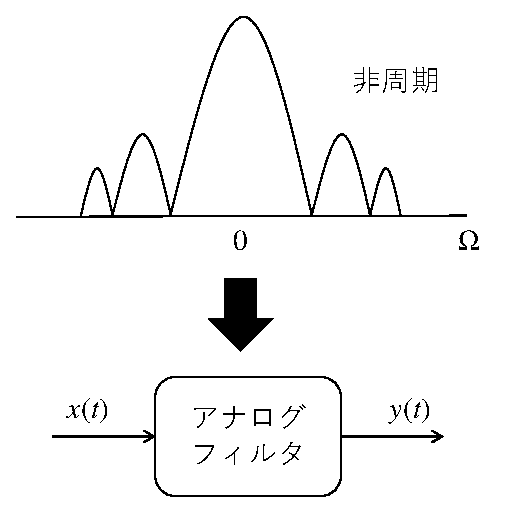
\includegraphics[width=4cm]{fig/zu-6-1.eps}
\end{center}
\caption{アナログフィルタ}
\label{fig:zu-6-1}
\end{figure}

一方,\index{でぃじたるふぃるた@ディジタルフィルタ}ディジタルフィルタは,図\ref{fig:zu-6-2}に示すように,\index{ADへんかんき@A-D変換器}A-D変換器によって生成されたディジタル信号を入力とし,ディジタル信号を出力するシステムである.必要があれば,出力段にD-A変換器を用いてアナログ信号に戻して,それを最終出力とする.このディジタルフィルタは,\index{でぃじたるかさんき@ディジタル加算器}ディジタル加算器,\index{じょうさんき@乗算器}乗算器,\index{ちえんき@遅延器}遅延器を用いて構成される.

\begin{figure}[H]
\begin{center}
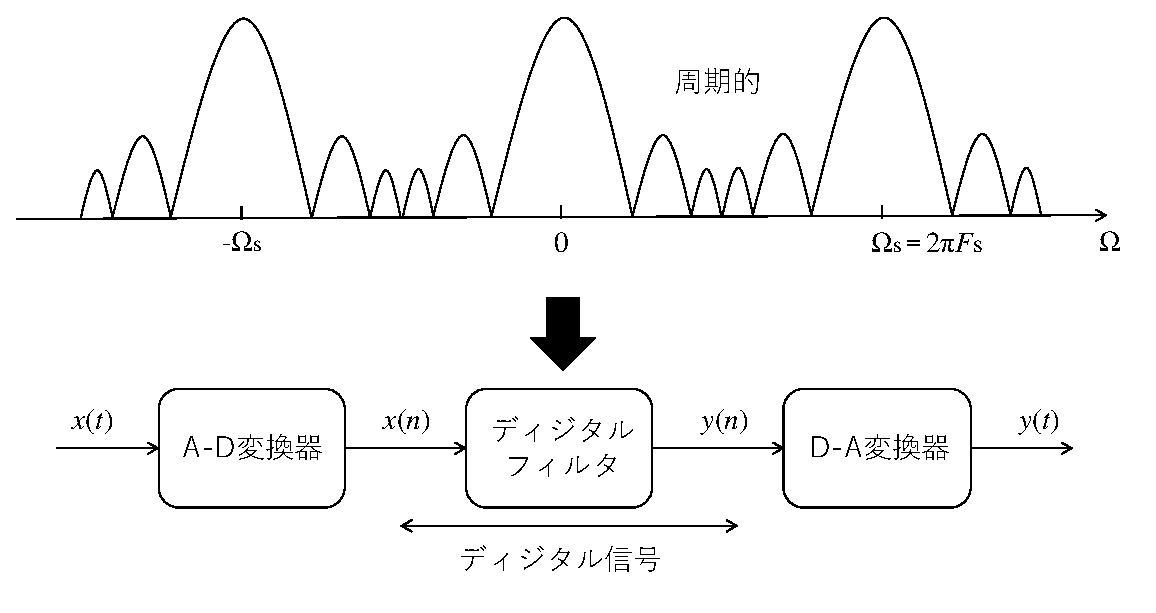
\includegraphics[width=10cm]{fig/zu-6-2.eps}
\end{center}
\caption{ディジタルフィルタ}
\label{fig:zu-6-2}
\end{figure}

\subsection{ディジタルフィルタの分類:\index{FIRふぃるた@FIRフィルタ}FIRフィルタと\index{IIRふぃるた@IIRフィルタ}IIRフィルタ}

%ディジタルフィルタは,FIRフィルタとIIRフィルタの2種類に分類される.この分類について述べる.

線形時不変システムの議論においても,FIR(\index{ゆうげんいんぱるす@有限インパルス}有限インパルス応答:Finit Inpulse Response)システムとIIR(無限インパルス応答:Infinit Inpulse Response)システムに分類されるが,ディジタルフィルタと同様にこの2つのシステムに分類することができる.

FIRシステムとして実現するか,IIRシステムとして実現するかによって,ディジタルフィルタの特徴が異なる.表\ref{table-6-1}に両者のちがいをまとめて示す.
実際の応用においては,これらの特徴を考慮して,まずはどちらのフィルタを用いるかを決定しなければならない.

\begin{table}
\caption{FIRフィルタとIIRフィルタとの比較}\label{table-6-1}
\begin{center}
\begin{tabular}{|c|c|c|}
\hline
 & FIRフィルタ & IIRフィルタ \\
\hline
安定性 & 常に安定 & 注意が必要 \\
\hline
直線位相特性 & 完全に実現可能 & 実現が困難 \\
\hline
伝達関数の次数 & 高い & 低い \\
\hline
\end{tabular}
\end{center}
\end{table}


\subsection{振幅特性による分類}

ディジタルフィルタの周波数特性$H(e^{j\omega})$は,\index{きょくざひょうひょうげん@極座標表現}極座標表現をすると,
\begin{equation}
H(e^{j\omega})=A(\omega)e^{j\omega}
\end{equation}
と書くことができるので,振幅特性$A(\omega)$と位相特性$e^{j\omega}$に分けて表現することができる.このフィルタの振幅特性$A(\omega)$のちがいによって,フィルタを分類する.信号を通過させる帯域(図\ref{fig:zu-6-3}において振幅1となる帯域)を通過域(pass band),信号を遮断する帯域を阻止域(stop band)というが,これらの配置から,
\begin{itemize}
\item 低域通過フィルタ (Low Pass Filter: LPF)
\item 高域通過フィルタ (High Pass Filter: HPF)
\item 帯域通過フィルタ (Band Pass Filter: BPF)
\item 帯域阻止フィルタ (Band Reject Filter: BRF)
\end{itemize}
と分類される.

高域通過フィルタは,ディジタルフィルタが取り扱える信号の最高の周波数$F_s/2$に対して通過域を持つという特性を持つ.帯域通過フィルタは$F_s/2$と直流($F=0$)に通過域がない.帯域阻止フィルタは帯域通過フィルタと逆の特性を持つ.

これらの特性は,FIRフィルタであれIIRフィルタであれ,実現が可能である.

\begin{figure}[H]
\begin{center}
%\includegraphics[width=9cm]{fig/zu-6-3.eps}
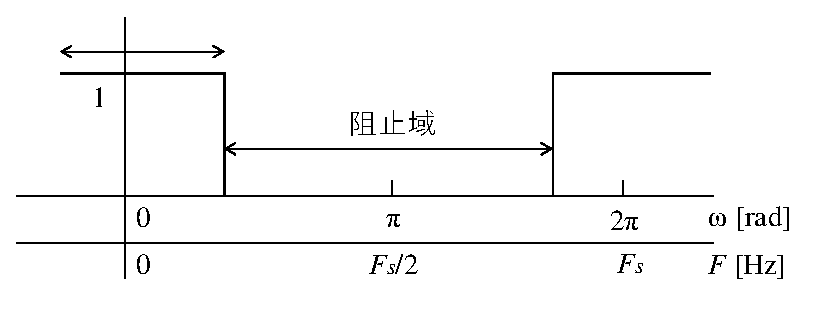
\includegraphics[width=9cm]{fig/zu-6-3-a.eps}

(a) LPF

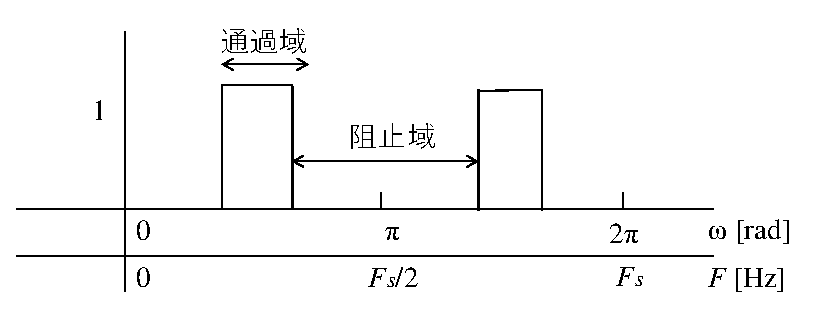
\includegraphics[width=9cm]{fig/zu-6-3-b.eps}

(b) BPF

\includegraphics[width=9cm]{fig/zu-6-3-c.eps}

(c) HPF

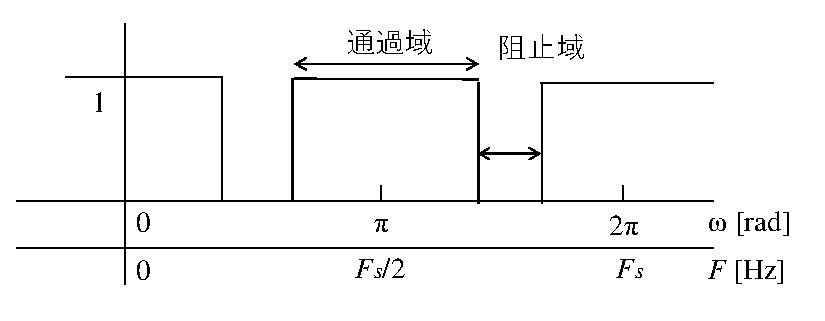
\includegraphics[width=9cm]{fig/zu-6-3-d.eps}

(d) BRF
\end{center}
\caption{振幅特性によるフィルタの分類}
\label{fig:zu-6-3}
\end{figure}


\subsection{位相特性による分類}

画像処理などへの応用においては,振幅特性だけでなく位相特性$\theta(\omega)$も重要である.そのような応用では,直線位相特性を持つ必要がある.直線位相特性とは,位相特性を角周波数$\omega$で微分した値
\begin{equation}
n_d=-\frac{d\theta(\omega)}{d\omega}
\end{equation}
が定数となる特性のことである.これは,位相特性の傾き$n_d$(群遅延量:group delay)が図\ref{fig:zu-6-4}のように一定であることを意味する.このような位相特性は,
\begin{equation}
\theta(\omega)=-n_d\omega-\theta_0
\label{eqn:eqn-6-3}
\end{equation}
と$\omega$に対して直線的な特性を持つ.ただし$\theta_0$は任意の定数である.

\index{ちょくせんいそうとくせい@直線位相特性}直線位相特性を持つディジタルフィルタを,直線位相フィルタ (linear phase filter)という.この特性の実現のためには,一般にFIRフィルタを用いる必要がある.

\begin{figure}[H]
\begin{center}
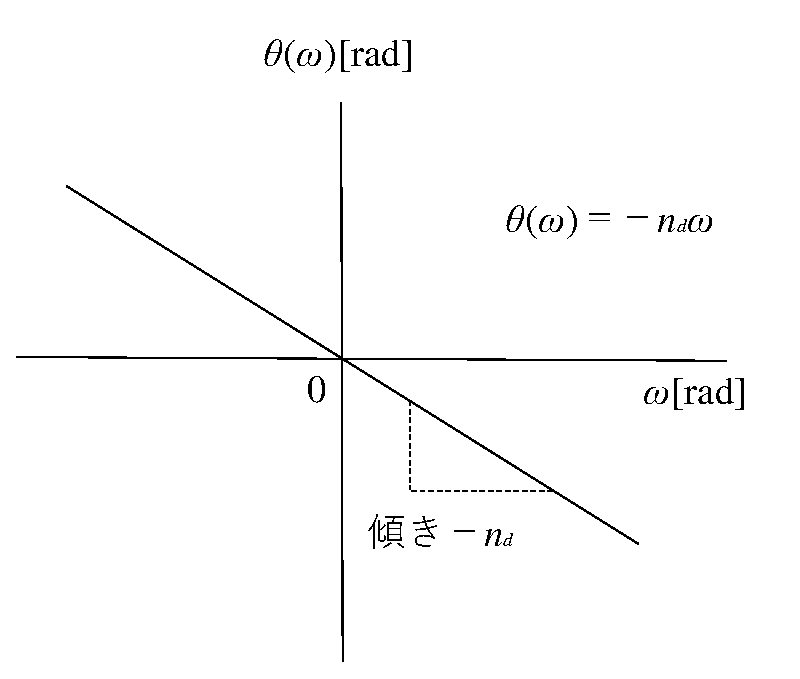
\includegraphics[width=8cm]{fig/zu-6-4.eps}
\end{center}
\caption{直線位相特性の一例}
\label{fig:zu-6-4}
\end{figure}

\section{理想フィルタと実際のフィルタ}

図\ref{fig:zu-6-3}の振幅特性は,厳密な表現をすることができない.そもそも実現可能なフィルタとはどのようなものであるかを,ここでは説明する.

\subsection{理想フィルタ}

\index{りそうふぃるた@理想フィルタ}理想フィルタは,振幅特性と位相特性に関して,以下に示す特徴を持つ.
\begin{itemize}
\item 通過域の振幅値は一定である.
\item 阻止域の振幅値は零である.
\item 通過域から阻止域に掛けて不連続に変化する.
\item 直線位相特性を持つ.
\end{itemize}
以上の条件をすべて満足するものを理想フィルタという.理想フィルタの振幅特性は図\ref{fig:zu-6-3}に示されるようなものであり,位相特性は図\ref{fig:zu-6-4}に示されるようなものである.実際には,振幅特性に関する条件を満足するフィルタは実現できないため,理想フィルタは実現不可能である.しかしながら,理想フィルタは理論的な考察を行う場合に重要な役割を持つ.

\subsection{実際のフィルタ}

図\ref{fig:zu-6-5}に示す振幅特性を例として,実際のフィルタ特性について説明をする.
%
まず,実際のフィルタは,理想フィルタと以下の点が異なる.

\begin{itemize}
\item 通過域の振幅値は一定ではなく,通過域誤差$\delta_p$を持つ.
\item 阻止域の振幅値は零ではなく,阻止域誤差$\delta_s$を持つ.
\item 通過域と阻止域との間に,過渡域(あるいは遷移域)なる帯域を持つ.
\end{itemize}

また,通過域の始まる周波数を通過域端周波数$F_p$,阻止域が始まる周波数を阻止域端周波数$F_r$という.

理想フィルタに近いほど,すなわち通過域誤差と阻止域誤差が小さく過渡域が狭いほど,高次の伝達関数が必要となり実現が複雑となる.加えて,帯域通過フィルタおよび帯域阻止フィルタの場合では,特性を規定するために通過域端周波数と阻止域端周波数をそれぞれ2つ指定する必要がある.

\begin{figure}[H]
\begin{center}
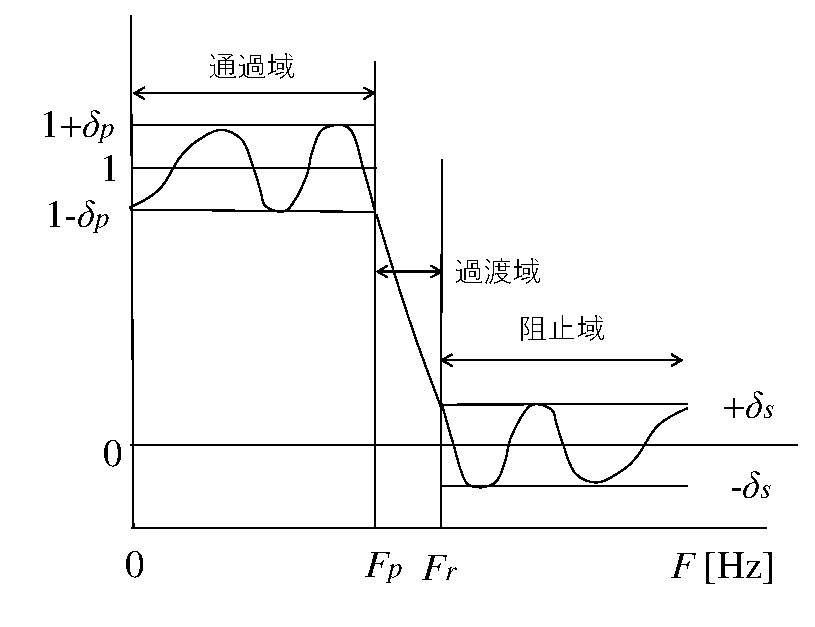
\includegraphics[width=8cm]{fig/zu-6-5.eps}
\end{center}
\caption{実際のフィルタの振幅特性}
\label{fig:zu-6-5}
\end{figure}



\section{直線位相フィルタ}

波形伝送や画像処理を行う際には,直線位相特性を持つフィルタを用いる必要がある.ここでは,FIRフィルタにより\index{ちょくせんいそうふぃるた@直線位相フィルタ}直線位相フィルタが容易に実現可能であることを説明する.

\subsection{直線位相の必要性}

図\ref{fig:zu-6-7}(c)に点線で表された信号$y(t)$を考える.この非正弦波信号$y(t)$は,図\ref{fig:zu-6-7}(a),(b)の2つの正弦波信号$x_1(t)$と$x_2(t)$に分解される.第\ref{chapter:6}章で述べたように,一般に非正弦波信号は正弦波信号の合成として表現される.また,位相特性は正弦波を入力した場合の位相(rad)のずれを表している.


\begin{figure}[H]
\begin{center}
%\includegraphics[width=10cm]{fig/zu-6-7.eps}
\begin{minipage}{.35\textwidth}
\begin{center}
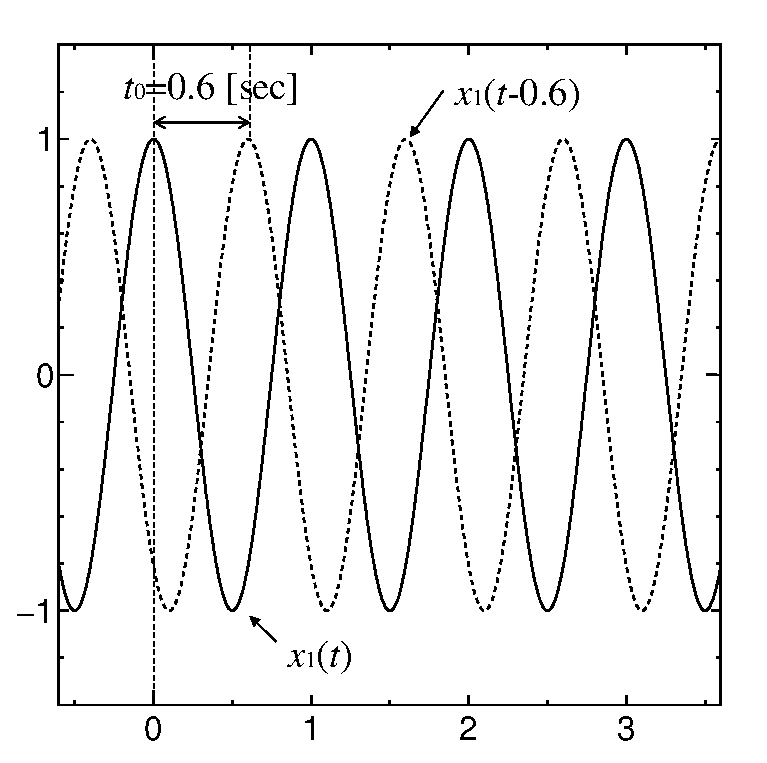
\includegraphics[width=.98\textwidth]{fig/zu-6-7-a.eps}

(a)
\end{center}
\end{minipage}
\begin{minipage}{.35\textwidth}
\begin{center}
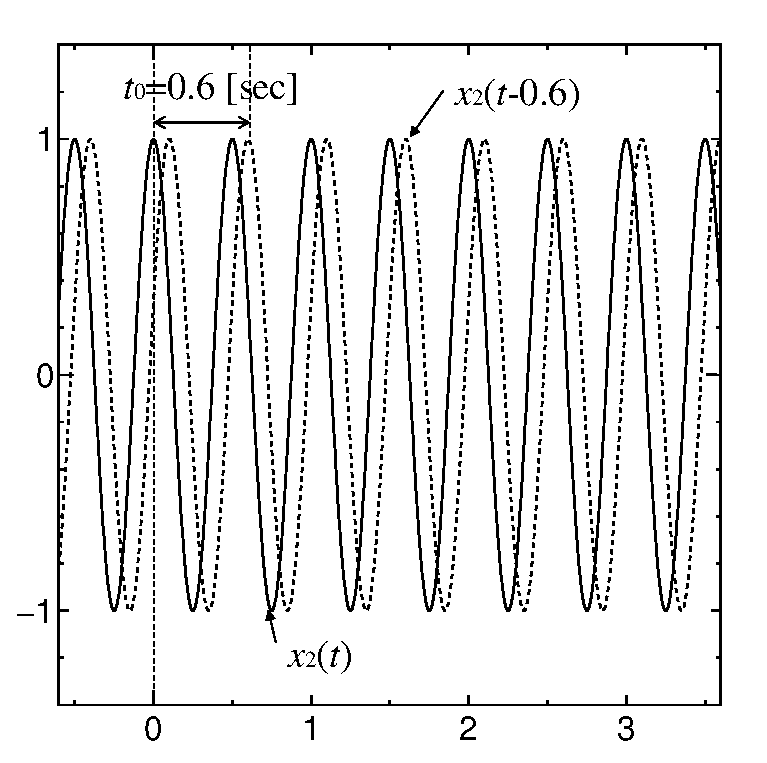
\includegraphics[width=.98\textwidth]{fig/zu-6-7-b.eps}

(b)
\end{center}
\end{minipage}\\[.5\baselineskip]
\begin{minipage}{.35\textwidth}
\begin{center}
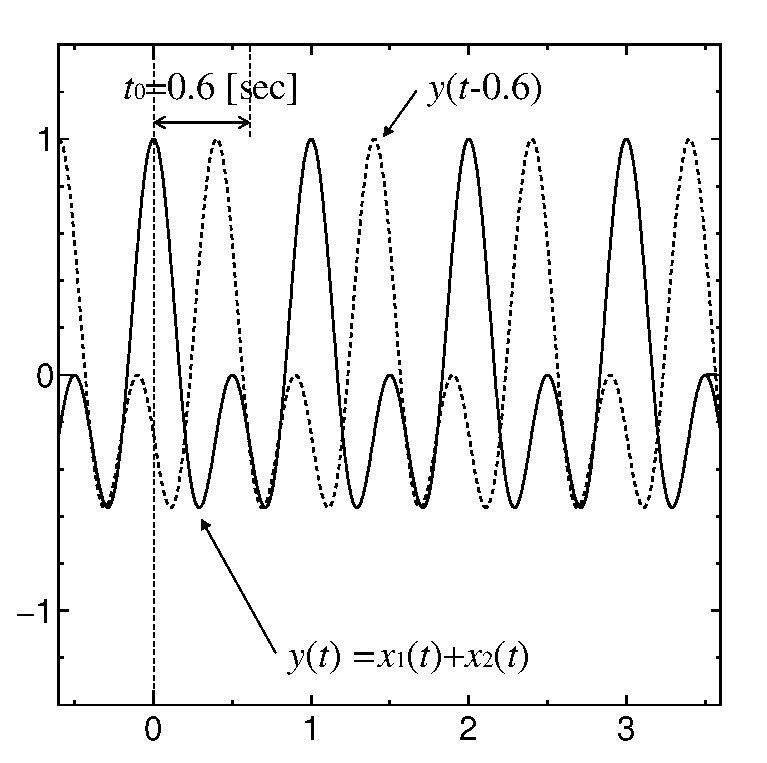
\includegraphics[width=.98\textwidth]{fig/zu-6-7-c.eps}

(c)
\end{center}
\end{minipage}
\end{center}\vskip.5\baselineskip
\caption{時間がずれた場合の信号例(一定時間$t_0$)}
\label{fig:zu-6-7}
\end{figure}


\subsubsection{位相ひずみ}

図\ref{fig:zu-6-7}における実線は,2つの正弦波信号がフィルタ処理によって同じ時間だけずれた信号である.また,図\ref{fig:zu-6-7}における破線は,その条件を満たさずに位相がずれた信号である.これらの例から,
\begin{itemize}
\item 正弦波のずれのちがいによって,合成される信号の形が大きく異なる
\item 各正弦波が同じ時間だけずれた場合,合成される信号は,時間シフト以外のひずみは生じない
\end{itemize}
ということがわかる.図\ref{fig:zu-6-7}における破線で示した例のように,位相のずれが原因で発生するひずみを位相ひずみという.直線位相特性は,この位相ひずみを回避できる特性である.

\subsubsection{位相ひずみの回避}

ここでは,直線位相特性により位相ひずみを回避できることを説明する.いま,信号$x_1(n)=\cos (\omega_1 n)$を周波数特性$H(e^{j\omega})=e^{j\theta (\omega )}$を持つシステムに入力すると,出力信号$y_1(n)$は,
\begin{equation}
y_1(n)=\cos (\omega_1 n + \theta (\omega_1))
\label{eqn:eqn-6-4}
\end{equation}
と与えられる.式(\ref{eqn:eqn-6-3})を式(\ref{eqn:eqn-6-4})に代入すると,
\begin{equation}
y_1(n)=\cos (\omega_1 n + n_d \omega_1 -\theta_0)
\label{eqn:eqn-6-5}
\end{equation}
となる.

ここで,簡単のため,$\theta (\omega )=-n_d \omega$を仮定するとき,式(\ref{eqn:eqn-6-5})は,

\begin{eqnarray}
y_1(n)&=&\cos (\omega_1 n - n_d \omega_1 ) \nonumber \\
 &=&\cos (\omega_1 (n - n_d)) \nonumber \\
 &=&x_1 ( n - n_d )
\label{eqn:eqn-6-6}
\end{eqnarray}\vskip.3\baselineskip

\noindent と整理される.この式は,単なる$n_d$サンプルの\index{じかんちえん@時間遅延}時間遅延を意味し,任意の周波数の正弦波信号に対して成り立つ.このことから,正弦波信号の合成として与えられる信号$y(n)$は,
\begin{equation}
y_1(n)=x ( n - n_d)
\label{eqn:eqn-6-7}
\end{equation}
と単なる入力信号$x(n)$の時間遅延をしたものとなり,位相ひずみは伴わないのである.

ここで,図\ref{fig:zu-2-2-1}に示すような平均処理における雑音除去を例として考える.$N$点の平均処理は直線位相を持ち,群遅延量$n_d = (N-1)/2$を持つ.したがって,図\ref{fig:zu-2-2-1}に示すような処理における時間のずれは$(N-1)/2$サンプルとなることを確認できる.

\begin{figure}[H]
\begin{center}
\begin{minipage}{.4\textwidth}
\begin{center}
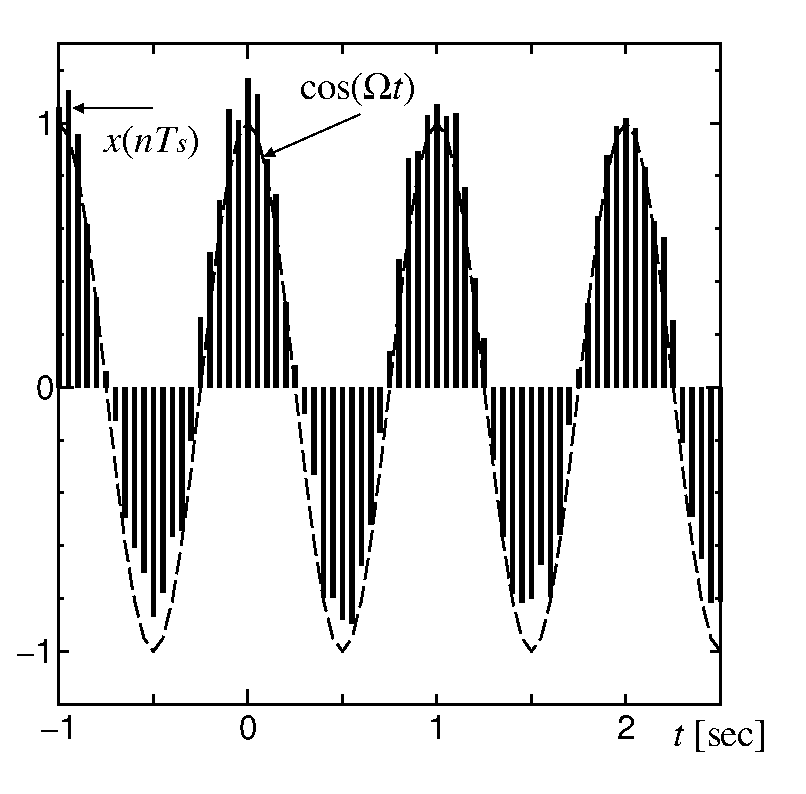
\includegraphics[width=.98\textwidth]{fig/zu-2-2-a.eps}

(a) 雑音を含んだ信号
\end{center}
\end{minipage}
\begin{minipage}{.4\textwidth}
\begin{center}
\includegraphics[width=.98\textwidth]{fig/zu-2-2-b.eps}

(b) 3点平均
\end{center}
\end{minipage}\\[.3\baselineskip]
\begin{minipage}{.4\textwidth}
\begin{center}
\includegraphics[width=4.5cm]{fig/zu-2-2-c.eps}

(c) 9点平均
\end{center}
\end{minipage}
\end{center}\vskip.3\baselineskip
\caption{平均処理による雑音の除去例($F=1$Hz,$F_s=20$Hz)}
\label{fig:zu-2-2-1}
\end{figure}



\subsection{直線位相フィルタ}

ここでは,FIRフィルタを用いることにより,直線位相特性を容易に実現できることを述べる.

因果性を満たすFIRフィルタの伝達関数$H(z)$は,
\begin{equation}
H(z)=\sum_{n=0}^{N-1}h(n)z^{-n}
\label{eqn:eqn-6-8}
\end{equation}
のように記述できる.ここで,実係数$h(n)$はインパルス応答である.また,$N-1$をフィルタの次数,$N$をタップ数またはインパルス応答の個数という.


\subsubsection{インパルス応答の対称性}

式(\ref{eqn:eqn-6-8})のFIRシステムが直線位相を持つための必要十分条件は,そのインパルス応答が図\ref{fig:zu-6-9}における4つの場合のいずれかの対称性を持つことである.すなわち,
\begin{enumerate}
\item 個数$N$が奇数であり,かつ偶対称$h(n)=h(N-n-1)$
\item 個数$N$が偶数であり,かつ偶対称$h(n)=h(N-n-1)$
\item 個数$N$が奇数であり,かつ奇対称$h(n)=-h(N-n-1)$
\item 個数$N$が偶数であり,かつ奇対称$h(n)=-h(N-n-1)$
\end{enumerate}

したがって,直線位相フィルタを実現するためには,図\ref{fig:zu-6-9}のいずれかの対称性を持つインパルス応答を使用すればよい.

\begin{figure}[H]
\begin{center}
\begin{minipage}[b]{.35\textwidth}
\begin{center}
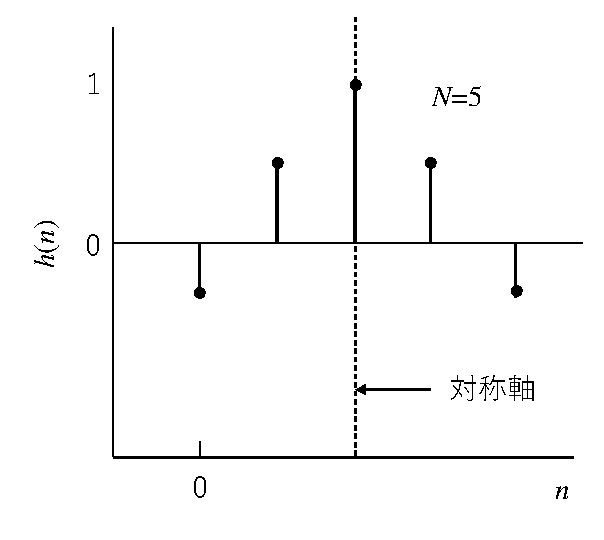
\includegraphics[width=.98\textwidth]{fig/zu-6-9-a.eps}

(a) 場合1
\end{center}
\end{minipage}
\begin{minipage}[b]{.35\textwidth}
\begin{center}
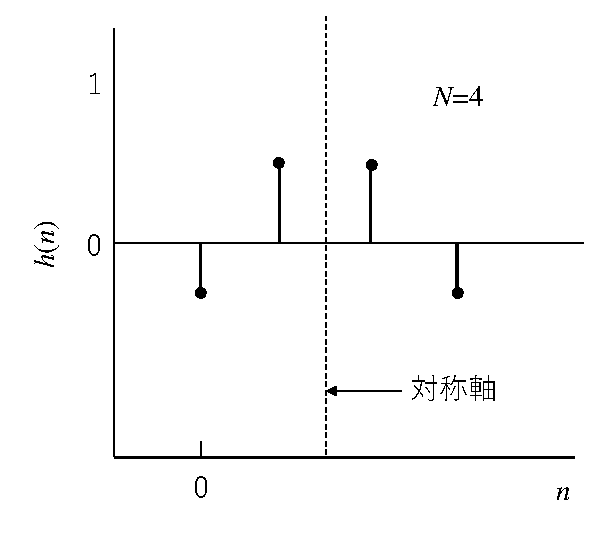
\includegraphics[width=.98\textwidth]{fig/zu-6-9-b.eps}

(b) 場合2
\end{center}
\end{minipage}\\[.3\baselineskip]
\begin{minipage}[b]{.35\textwidth}
\begin{center}
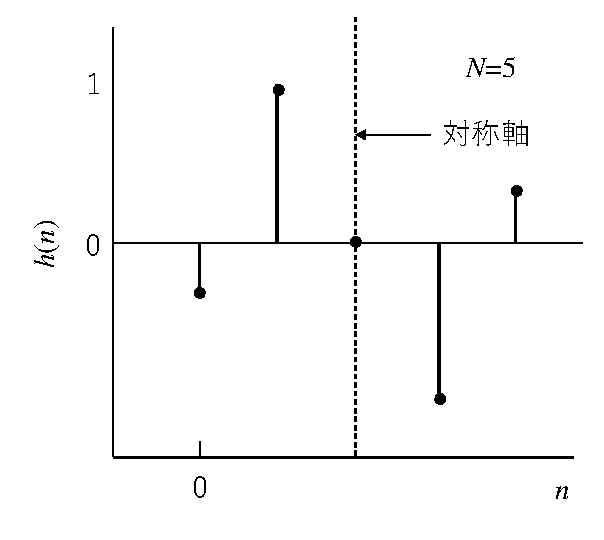
\includegraphics[width=.98\textwidth]{fig/zu-6-9-c.eps}

(c) 場合3
\end{center}
\end{minipage}
\begin{minipage}[b]{.35\textwidth}
\begin{center}
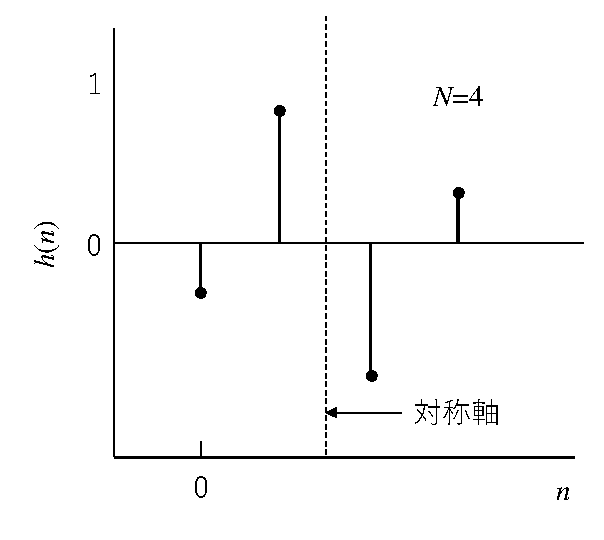
\includegraphics[width=.98\textwidth]{fig/zu-6-9-d.eps}

(d) 場合4
\end{center}
\end{minipage}
\end{center}\vskip.3\baselineskip
\caption{インパルス応答の対称性}
\label{fig:zu-6-9}
\end{figure}

\subsubsection{直線位相フィルタの周波数特性}


式(\ref{eqn:eqn-6-8})の伝達関数を持つFIRフィルタが直線位相特性を持つとき,その周波数特性
\begin{equation}
H(e^{j\omega}) = A(\omega)e^{j\theta (\omega )}
\end{equation}
は,表\ref{table:table-6-21}に示すように整理される.ここで,$A(\omega )$は振幅特性,$\theta (\omega ) $は位相特性である.

このことから,まず,位相特性はインパルス応答の個数$N$と対称性により決定することがわかる.次に,位相特性も,インパルス応答の対称性の影響を強く受けることがわかる.

\begin{table}[H]
\caption{直線位相フィルタの周波数特性}
\label{table:table-6-21}
\begin{center}
\begin{tabular}{|c|c|c|c|c|}
\hline
場合 & $h(n)$ & $N$ & 位相 $\theta (\omega)$ & 振幅 $A(\omega)$ \\
\hline
1 & 偶対称 & 奇数 & $-\omega(N-1)/2$ & $\displaystyle \sum_{n=0}^{(N-1)/2}a_n \cos (\omega n)$ \\
\hline
2 & 偶対称 & 偶数 & $-\omega(N-1)/2$ & $\displaystyle \sum_{n=0}^{(N-1)/2}b_n \cos (\omega (n-1/2))$ \\
\hline
3 & 奇対称 & 奇数 & $-\omega(N-1)/2+\pi/2$ & $\displaystyle \sum_{n=0}^{(N-1)/2}a_n \sin (\omega n)$ \\
\hline
4 & 偶対称 & 偶数 & $-\omega(N-1)/2+\pi/2$ & $\displaystyle \sum_{n=0}^{(N-1)/2}b_n \sin (\omega (n-1/2))$ \\
\hline
\end{tabular}
\end{center}
\end{table}

\subsubsection{振幅特性の制約}

直線位相フィルタを使用する場合に大切な振幅特性の制約について述べる.直線位相フィルタの振幅特性は,インパルス応答の対称性により図\ref{fig:zu-6-11}に示すような制約を受ける.すなわち,
\begin{enumerate}
\item Case 1: $\omega = \pi$で偶対称な特性を持ち,\index{ていいきふぃるた@低域フィルタ}低域フィルタ(LPF),\index{たいいきふぃるた@帯域フィルタ}帯域フィルタ(BPF),および\index{こういきふぃるた@高域フィルタ}高域フィルタ(HPF)をすべて設計できる.
\item Case 2: 奇対称な振幅特性を有する場合,HPFを設計できない.
\item Case 3: 振幅特性が奇対称でかつ$\omega=0$で零値である場合,LPFおよびHPFを設計できない.
\item Case 4: 振幅特性が$\omega=0$で零値である場合,LPFを設計できない.
\end{enumerate}
のように場合分けできる.

\begin{figure}[H]
\begin{center}
\begin{minipage}{.35\textwidth}
\begin{center}
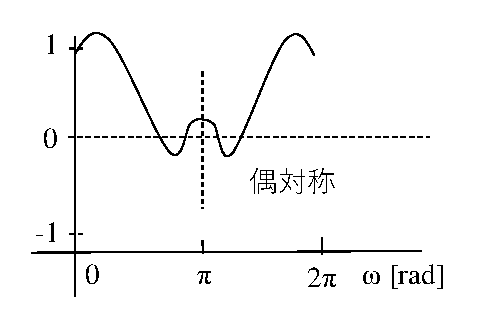
\includegraphics[width=.98\textwidth]{fig/zu-6-11-a.eps}

(a) 場合1
\end{center}
\end{minipage}
\begin{minipage}{.35\textwidth}
\begin{center}
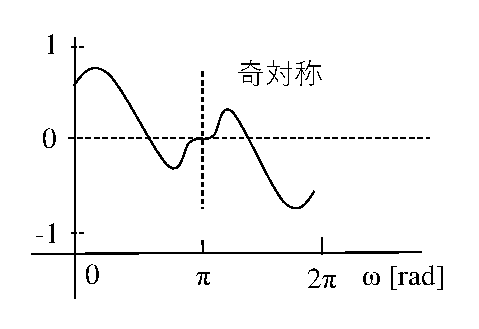
\includegraphics[width=.98\textwidth]{fig/zu-6-11-b.eps}

(b) 場合2
\end{center}
\end{minipage}\\[.3\baselineskip]
\begin{minipage}{.35\textwidth}
\begin{center}
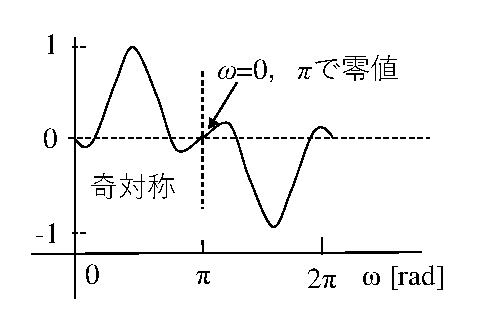
\includegraphics[width=.98\textwidth]{fig/zu-6-11-c.eps}

(c) 場合3
\end{center}
\end{minipage}
\begin{minipage}{.35\textwidth}
\begin{center}
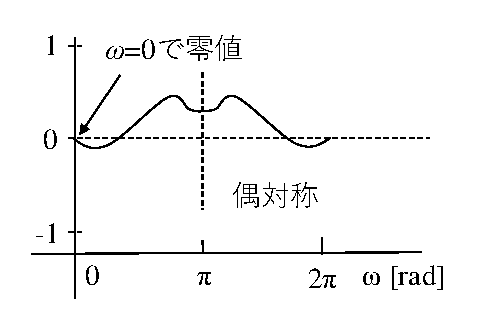
\includegraphics[width=.98\textwidth]{fig/zu-6-11-d.eps}

(d) 場合4
\end{center}
\end{minipage}
%\includegraphics[width=10cm]{fig/zu-6-11.eps}
\end{center}\vskip.3\baselineskip
\caption{直線位相フィルタの振幅特性}
\label{fig:zu-6-11}
\end{figure}

\subsection{窓関数によるFIRフィルタの設計}

フィルタを実際に使用する場合,所望の周波数特性を持つ伝達関数を決定する必要がある.ここでは,窓関数法と呼ばれる直線位相特性を持つFIRフィルタの伝達関数の設計法を概説する.

\noindent{\bf 手順1:所望の振幅特性を決める.}

たとえば,図\ref{fig:zu-6-12}(a)に示される振幅特性を実現するものと考える.


\noindent{\bf 手順2:インパルス応答を求める.}

図\ref{fig:zu-6-12}(a)に示される振幅特性の場合,図\ref{fig:zu-6-12}(a)を逆離散時間フーリエ変換し,図\ref{fig:zu-6-12}(b)に示すような所望の振幅特性に対応するインパルス応答$h_d(n)$を求める.ただし,インパルス応答$h_d(n)$は無限の区間に存在するため,このまま直接使用することはできない.

\noindent{\bf 手順3:$N$点の窓関数$w(n)$を掛けて,有限な範囲で切り出す.}

直線位相を持つようにインパルス応答の対称性を考慮して,図\ref{fig:zu-6-12}(c)のように切り出す.しかし,このフィルタは負の時間でインパルス応答を持つため,因果性を満たしていない.

\noindent{\bf 手順4:\index{いんがせい@因果性}因果性を満たすように,インパルス応答を時間シフトする.}

因果性を満たすように,非負の時間でインパルス応答が存在するように時間シフトをして,図\ref{fig:zu-6-12}(d)を得る.このインパルス応答を持つフィルタの振幅特性を再び計算すると図\ref{fig:zu-6-12}(e)のようになり,これは図\ref{fig:zu-6-12}(a)に近い特性が得られることがわかる.

当然ではあるが,使用する窓関数の種類や,窓関数の大きさ$N$(インパルス応答の個数)によって,実現される振幅特性が異なる.

\begin{figure}[H]
\begin{center}
\begin{minipage}{.4\textwidth}
\begin{center}
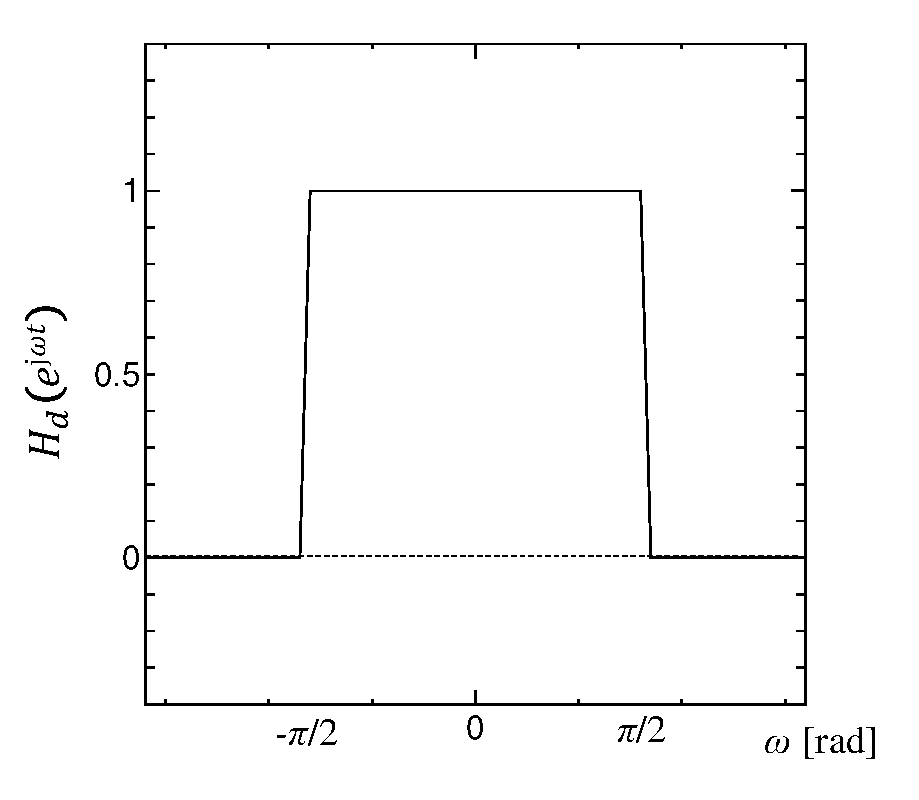
\includegraphics[width=.98\textwidth]{fig/zu-6-12-a.eps}

(a) 所望の特性
\end{center}
\end{minipage}
\begin{minipage}{.38\textwidth}
\begin{center}
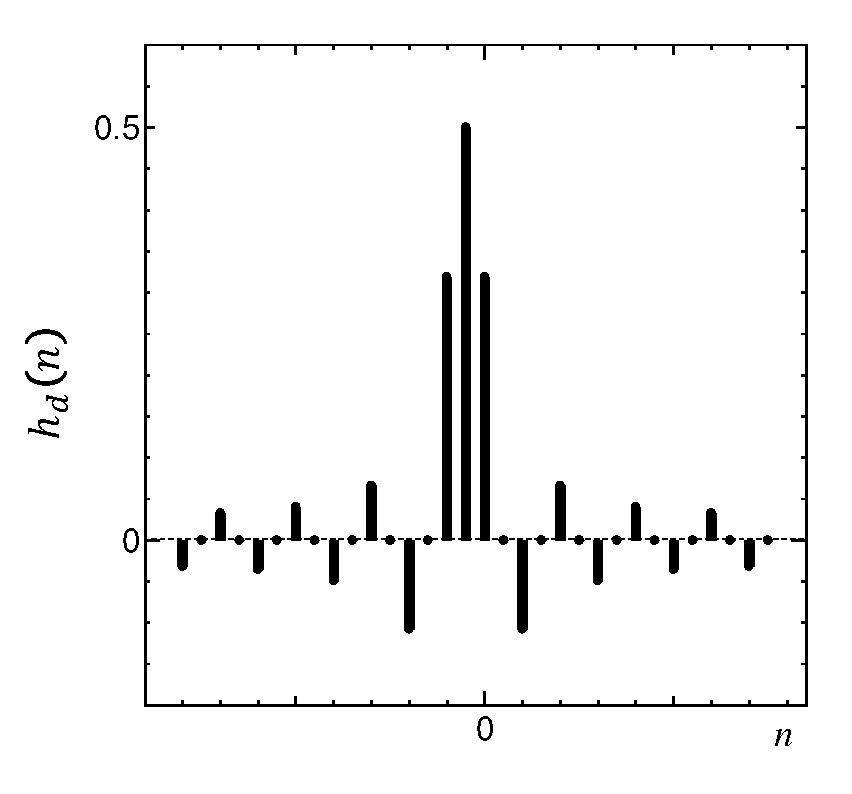
\includegraphics[width=.98\textwidth]{fig/zu-6-12-b.eps}

(b) 所望のインパルス応答
\end{center}
\end{minipage}\\[.3\baselineskip]
\begin{minipage}{.38\textwidth}
\begin{center}
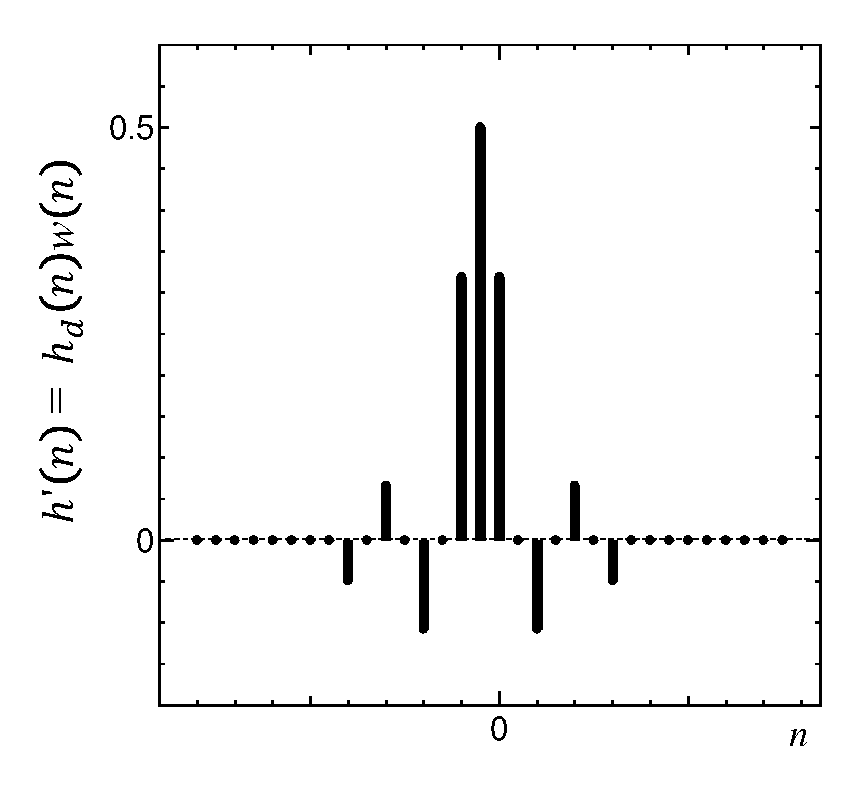
\includegraphics[width=.98\textwidth]{fig/zu-6-12-c.eps}

(c) 切り出したインパルス応答
\end{center}
\end{minipage}
\begin{minipage}{.38\textwidth}
\begin{center}
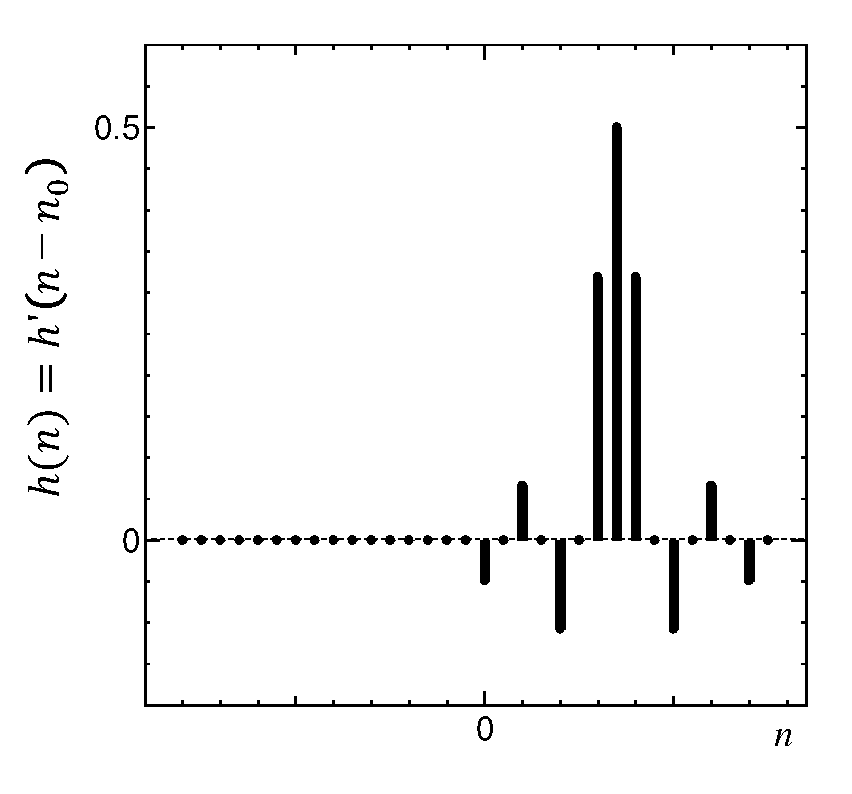
\includegraphics[width=.98\textwidth]{fig/zu-6-12-d.eps}

(d) シフトされたインパルス応答
\end{center}
\end{minipage}\\[.3\baselineskip]
\begin{minipage}{.38\textwidth}
\begin{center}
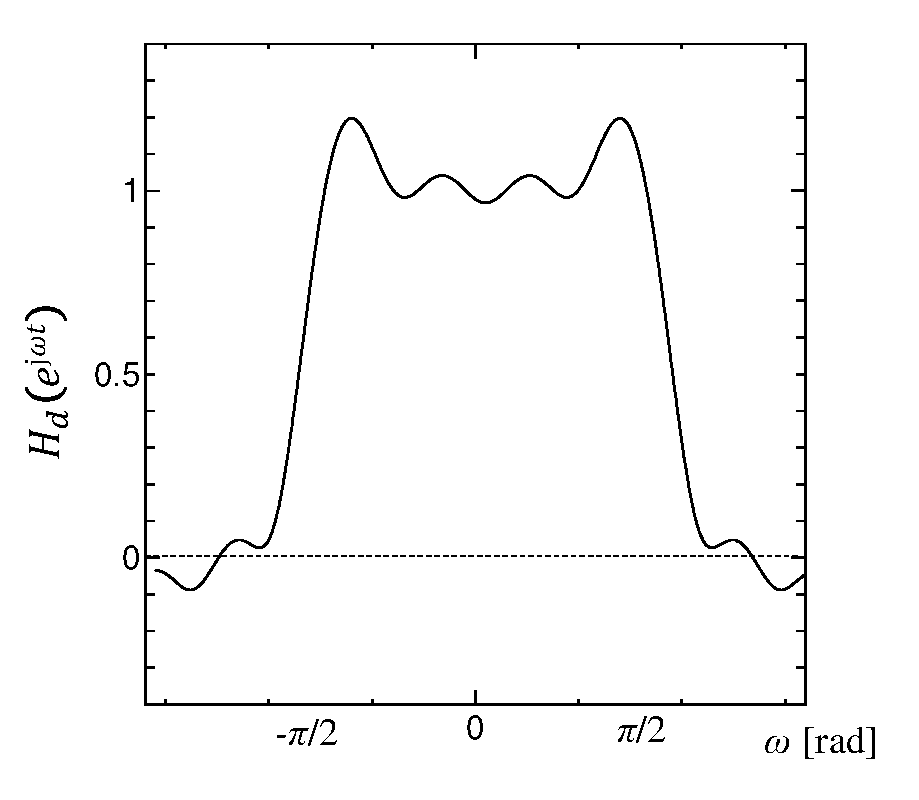
\includegraphics[width=.98\textwidth]{fig/zu-6-12-e.eps}

(e) 実現された特性
\end{center}
\end{minipage}
%\includegraphics[width=10cm]{fig/zu-6-12.eps}
\end{center}\vskip.3\baselineskip
\caption{直線位相フィルタの振幅特性}
\label{fig:zu-6-12}
\end{figure}

\clearpage 

\section{ディジタルフィルタの構成法}

ディジタルフィルタの構成には種々の方法がある.ここでは,代表的な構成法を説明する.

\subsection{FIRフィルタ}

例として,次式に示す伝達関数を考えるものとする.
\begin{equation}
H(z)=\sum_{n=0}^{N-1}h(n)z^{-n}
\label{eqn:eqn-6-81}
\end{equation}

この伝達関数は,$N=4$を例にすると,図\ref{fig:zu-6-14}(a)のような直接型構成または図\ref{fig:zu-6-14}(b)のような転置型構成のように構成される.この2つのちがいは遅延器$z^{-1}$の位置であるが,同じ入出力関係を持つことは容易に確認することができる.

また,FIRフィルタが直線位相特性を持つ場合,そのインパルス応答は対称性を持つ.その場合は約半分の乗算値が同じ値となるので,FIRフィルタの実現の際に乗算器の数を半分に低減することができる.

\begin{figure}[H]
\begin{center}
\begin{minipage}{.4\textwidth}
\begin{center}
\includegraphics[width=.98\textwidth]{fig/zu-6-14-a.eps}

(a) 直接型構成
\end{center}
\end{minipage}
\begin{minipage}{.4\textwidth}
\begin{center}
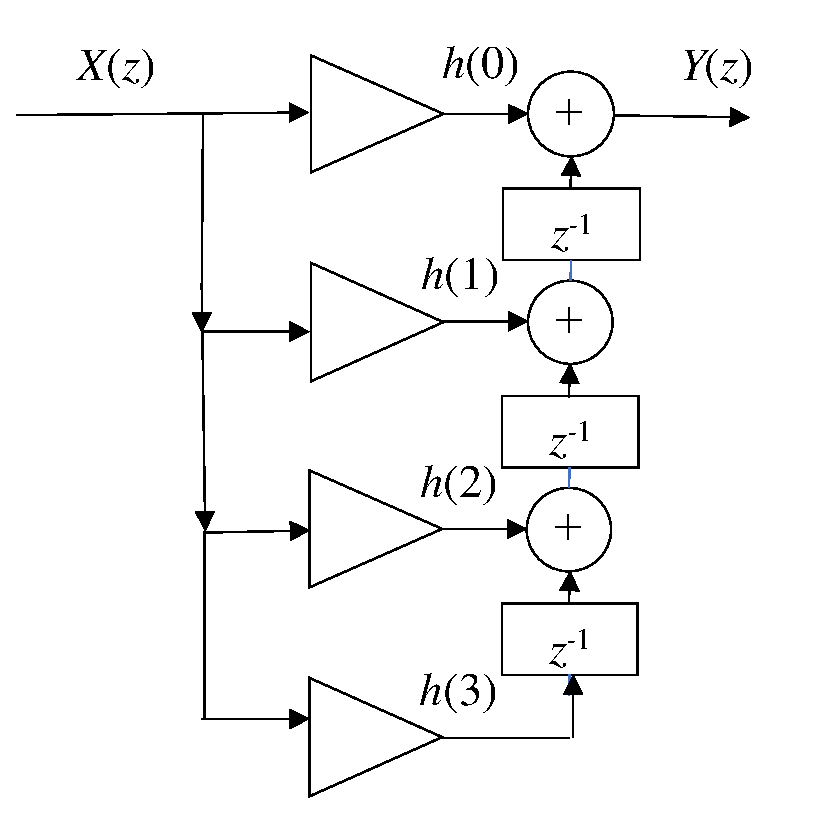
\includegraphics[width=.98\textwidth]{fig/zu-6-14-b.eps}

(b) 転置型構成
\end{center}
\end{minipage}
\end{center}\vskip.5\baselineskip
\caption{直線位相フィルタの振幅特性}
\label{fig:zu-6-14}
\end{figure}

\subsection{IIRフィルタ}

IIRフィルタの伝達装置として,
\begin{equation}
H(z)=\displaystyle \frac{\displaystyle \sum_{k=0}^{M}a_kz^{-k}}{\displaystyle 1+\sum_{k=1}^{N}b_kz^{-k}}
\label{eqn:eqn-6-12}
\end{equation}
を考える.この伝達関数については,$M=N=3$の場合,図\ref{fig:zu-6-16-1}~\ref{fig:zu-6-16-3}に示すような3種類のいずれを用いてもよい.この図\ref{fig:zu-6-16-1}ならびに図\ref{fig:zu-6-16-2}の構成をIIRフィルタの直接型構成,図\ref{fig:zu-6-16-3}をIIRフィルタの転置型構成という.

ここで,図\ref{fig:zu-6-14}(a)ならびに図\ref{fig:zu-6-14}(b)の構成なるIIRフィルタの直接型構成が同じ特性を持つフィルタであることを示す.式(\ref{eqn:eqn-6-12})の伝達関数を

\begin{eqnarray}
H(z)&=&\displaystyle \frac{\displaystyle \sum_{k=0}^{M}a_kz^{-k}}{\displaystyle 1+\sum_{k=1}^{N}b_kz^{-k}} \nonumber \\
 &=&\frac{N(z)}{D(z)} \nonumber \\
 &=&N(z)\frac{1}{D(z)} \\
 &=&\frac{1}{D(z)}N(z)
\label{eqn:eqn-6-13}
\end{eqnarray}\vskip.3\baselineskip

\noindent と書くことができる.このことは$H_1(z)=N(z)$,$H_2(z)=1/D(z)$なる2つのフィルタの縦続的構成であることを解釈できるだけでなく,$H_1(z)$と$H_2(z)$との順番を入れ替えることができることを意味する.その結果,2つのフィルタは遅延器を共通に使用できることから.遅延器の個数を低減することが可能となる.

遅延器を少なくすることができるという理由で,図\ref{fig:zu-6-16-2}の直接型構成のほうが,図\ref{fig:zu-6-16-1}の直接型構成と比較して広く利用されている.
また,図\ref{fig:zu-6-16-3}の\index{てんちがたこうせい@転置型構成}転置型構成は,FIRフィルタの転置型構成と同様に遅延器の位置を移動したものである.その結果,遅延器を共通に使用することができることから,遅延器の個数を低減することができる.



\begin{figure}[H]
\begin{center}
\begin{minipage}{.8\textwidth}
\begin{center}
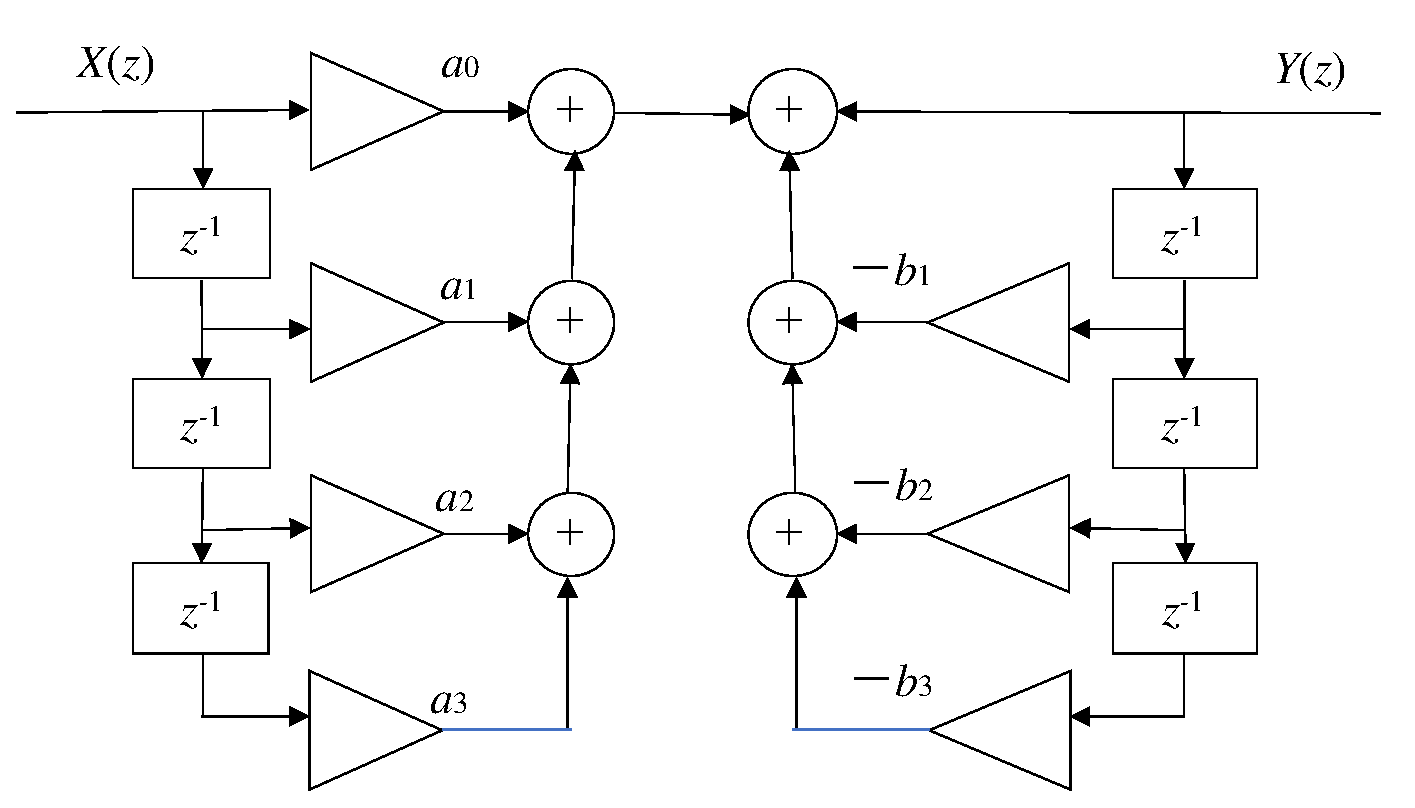
\includegraphics[width=\textwidth]{fig/zu-6-16-a.eps}
\end{center}
\end{minipage}
\end{center}
\caption{IIRフィルタの構成(直接型構成-I)}
\label{fig:zu-6-16-1}
\end{figure}

\begin{figure}[H]
\begin{center}
\begin{minipage}{.7\textwidth}
\begin{center}
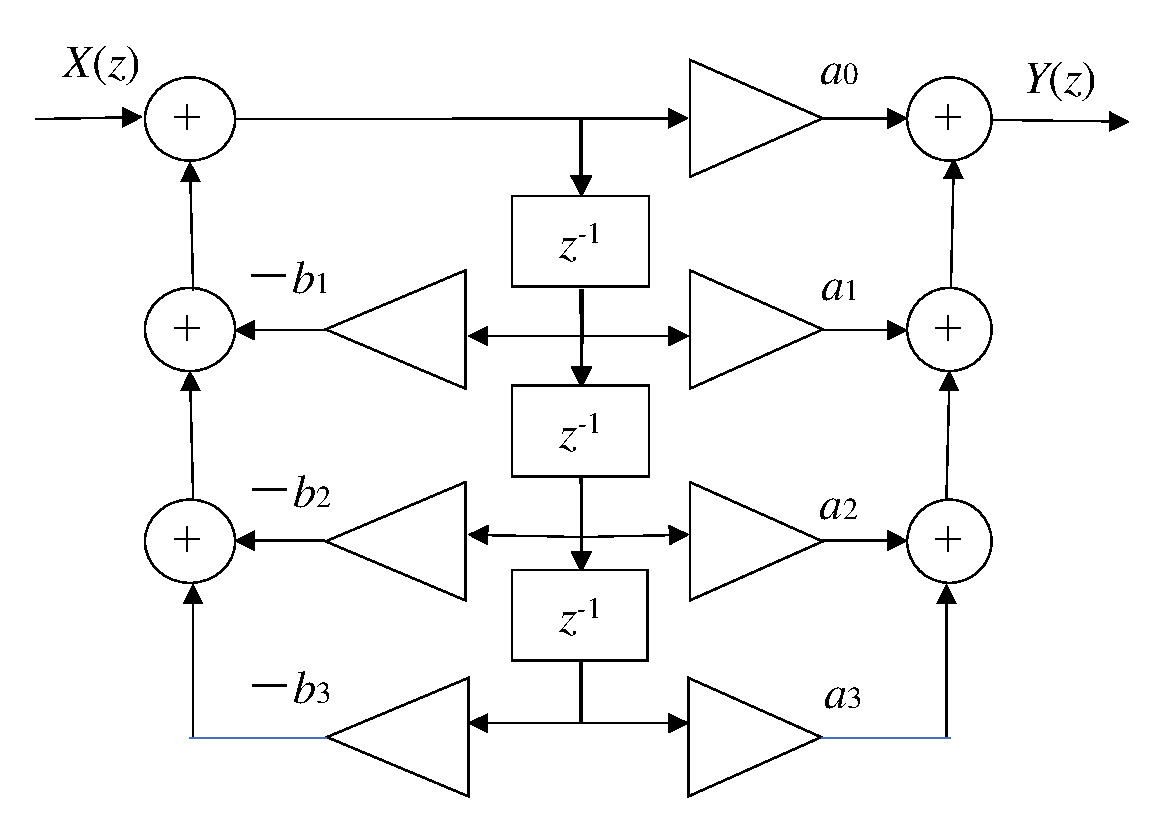
\includegraphics[width=\textwidth]{fig/zu-6-16-b.eps}
\end{center}
\end{minipage}
\end{center}
\caption{IIRフィルタの構成(直接型構成-II)}
\label{fig:zu-6-16-2}
\end{figure}

\begin{figure}[H]
\begin{center}
\begin{minipage}{.7\textwidth}
\begin{center}
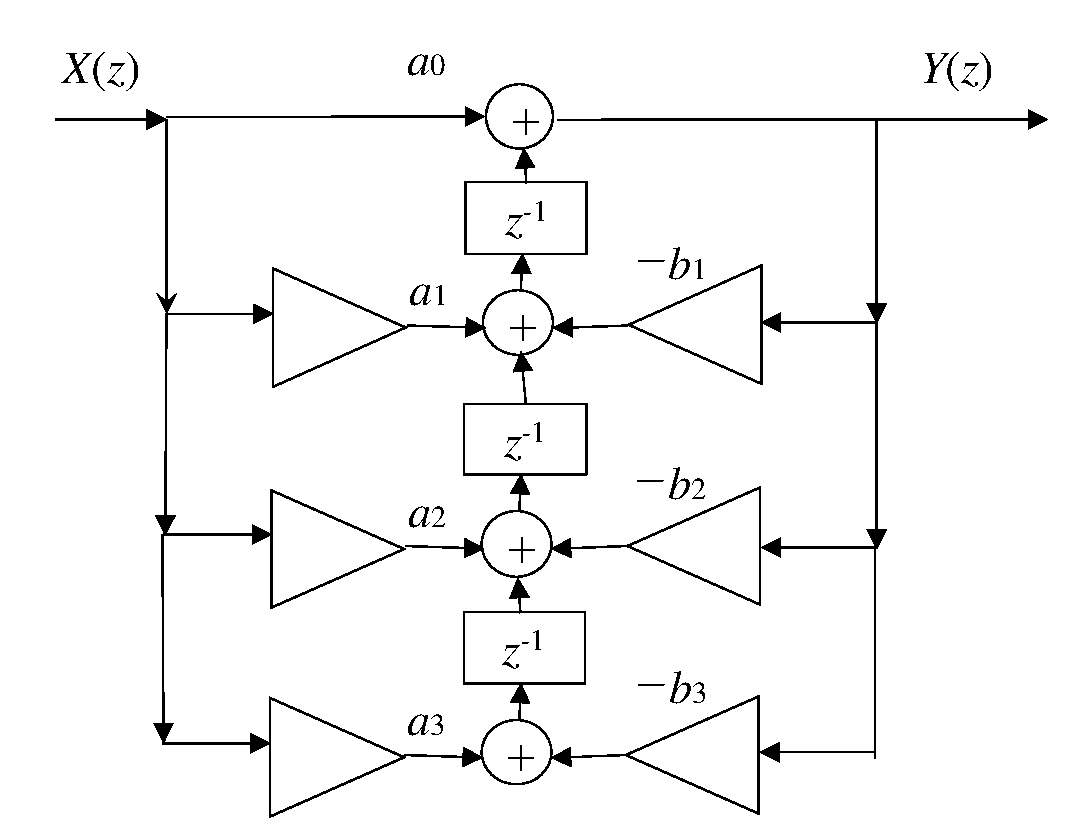
\includegraphics[width=\textwidth]{fig/zu-6-16-c.eps}
\end{center}
\end{minipage}
\end{center}
\caption{IIRフィルタの構成(転置型構成)}
\label{fig:zu-6-16-3}
\end{figure}


\subsection{IIRフィルタの縦続型構成}

高次のIIRフィルタを実際に構成する場合には,ここで説明する\index{じゅうぞくがたこうせい@縦続型構成}縦続型構成が最も広く用いられている.

式(\ref{eqn:eqn-6-12})を2次の伝達関数で次式のように分解する.
\begin{equation}
H(z)=\displaystyle H_0 \prod_{k=1}^{L}\frac{a_{0k}+a_{1k}z^{-1}+a_{2k}z^{-2}}{1+b_{1k}z^{-1}+b_{2k}z^{-2}}
\end{equation}
ただし,$H_0$は定数であり,$L$は整数である.たとえば,式(\ref{eqn:eqn-6-12})において,$M=N=5$ならば$L=(N+1)/2=3$,$M=N=6$ならば$L=N/2=3$である.

この表現は,図\ref{fig:zu-6-18}に示すように,2次の伝達関数の縦続型構成として高次の伝達関数を実現できることを意味する.したがって,伝達関数の次数にかかわらず,常に2次の伝達関数の組合せとしてフィルタを実現することができる.

ところで,2次を最低次数として因数分解する理由は,実係数を一般的に維持する最低次数が2次であることによる.各2次の伝達関数は,図\ref{fig:zu-6-16-1}~\ref{fig:zu-6-16-3}を用いて実現することができる.
伝達関数を部分分数展開し,低次の伝達関数の和の形式で表現することもでき,その場合は並列型構成を与える.

\begin{figure}[H]
\begin{center}
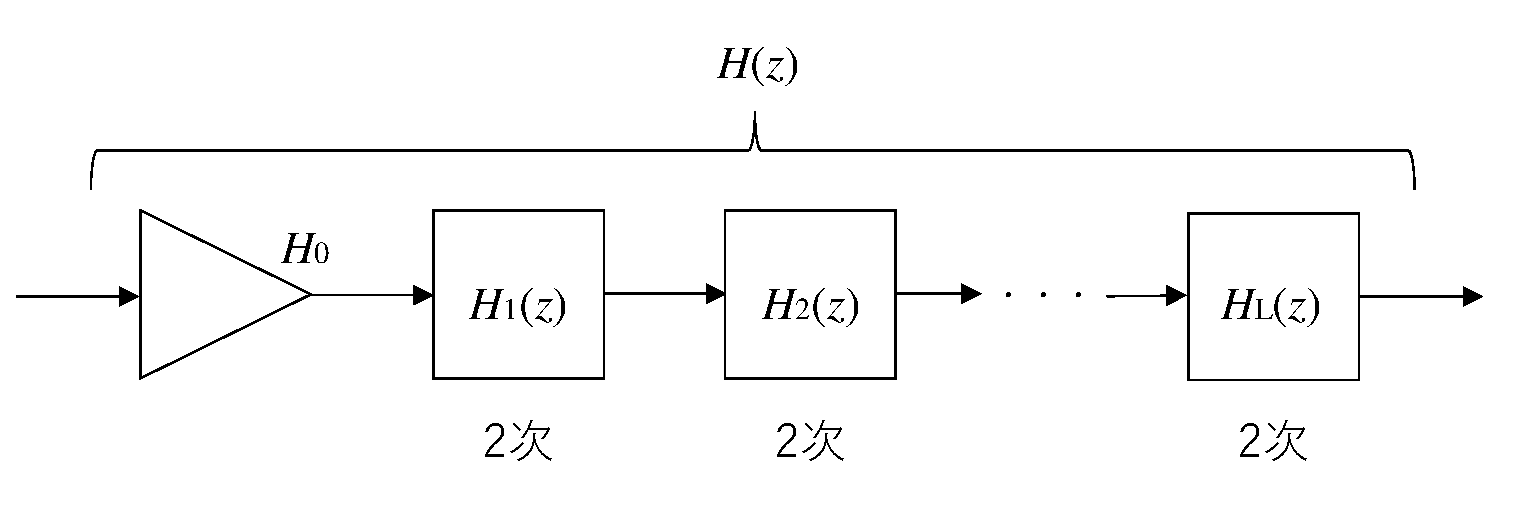
\includegraphics[width=.8\textwidth]{fig/zu-6-18.eps}
\end{center}
\caption{IIRフィルタの縦続型構成}
\label{fig:zu-6-18}
\end{figure}


\section*{演習問題}

\subsection*{問題\ref{chapter:11}.1}

伝達関数$H(z)=a+bz^{-1}+bz^{-2}+az^{-3}$について,2個の乗算器による\index{はーどうぇあこうせい@ハードウェア構成}ハードウェア構成図を示せ.

%\subsection*{問題\ref{chapter:11}.2}



